



%\section{Overview}

In the field of Information Retrieval \cite{Manning:2008:IIR:1394399}, there are techniques being widely used in several applications. They can be considered as a basic and indispensable part of a knowledge mining system. Throughout this deliverable some techniques are utilized in different similarity computation algorithms and thus it is worth conducting a review of them. Among others, Term-Document Matrix, Cosine Similarity, Latent Semantic Analysis and Jaccard Index are going to be briefly recalled due to their popularity. Furthermore, later in the chapter we also provide a brief introduction to a graph algorithm \cite{Jeh:2002:SMS:775047.775126}, which has been exploited to compute the similarity among OSS projects \cite{NDRDSEAA2018}.

%This section presents an overview of existing approaches that have been devised over the last decade to detect similar software systems. To this end a mathematical background, which is common to knowledge mining systems, is discussed in Sec. \ref{sec:mathBackground}. %Section \ref{sec:overview} presents an overview of existing software similarity measurement techniques.

%The and they serve as a base for further presentation.

%%%%%%%%%%%%%%%%%%%%%%%%%%%%%%%%%%%%%%%%%%%%%%%%%%%%%%%%%%

%\section{String-Based}

%Text similarity measures play an increasingly important role in text related research and applications in tasks such as information retrieval, text classification, document clustering, topic detection, topic tracking, questions generation, question answering, essay scoring, short answer scoring, machine translation, text summarization and others. Finding similarity between words is a fundamental part of text similarity which is then used as a primary stage for sentence, paragraph and document similarities. There two way in which words can be similar each other, lexically if they share sequences of characters similar and  semantically if are used in the same context, used in the same way and so on. 

%The world of lexical similarity con be divided in two categories: character-based and word-based. To better understand what character-based means, here one of the most well known technique: Levenshtein distance.

%\section{Levenshtein distance}
% Levenshtein distance defines distance between two strings by counting the minimum number of operations needed to transform one string into the other, where an operation is defined as an insertion, deletion, or substitution of a single character, or a transposition of two adjacent characters.
%
%This is an example:
%
%\begin{itemize}
%    \item kitten to sitten (substitution of "s" for "k").
%    \item sitten to sittin (substitution of "i" for "e").
%    \item sittin to sitting (insertion of "g" at the end).
%\end{itemize}
%
%Moving to the word-based,  the word or string similarity measures operate on string sequences and character composition. A string metric is a metric that measures similarity or dissimilarity (distance) between two text strings for approximate string matching or comparison.




\section{Term-Document Matrix} \label{sec:TDM}
In Natural Language Processing \cite{Collobert:2011:NLP:1953048.2078186}, a term-document matrix (TDM) is used to represent the relationships between words and documents \cite{Turney:2010:FMV:1861751.1861756}. In a TDM, each row corresponds to a document and each column corresponds to a term. A cell in the TDM represents the weight of a term in a document. The most common weighting scheme used in document retrieval is the \emph{term frequency-inverse document frequency (tf-idf)} function \cite{Reed:2006:TNT:1193211.1193734}. If we consider a set of $n$ documents $D=(d_{1},d_{2},..,d_{n})$ and a set of terms $t=(t_{1},t_{2},..,t_{r})$ then the representation of a document $d \in D $ is vector $\vec{\delta}=(w_{1}^{d},w_{2}^{d},..,w_{r}^{d})$, where the weight $w_{k}^{d}$ of term $k$ in document $d$ is computed using the {\em tf-idf} function \cite{Ramos1999}:

\begin{equation} \label{tfidf} %\nonumber 
w_{k}^{d} =tf\cdot idf(k,d,D)= f_{k}^{d}\cdot log\frac{n}{\left | \left \{ d\in D: t_{k} \in d \right \} \right |} 
\end{equation}

where $f_{k}^{d}$ is the frequency of term $t_{k}$ in document $d$.

Another common weighting scheme uses only the frequency of terms in documents for cells in TDM, \ie the number of occurrence of a term in a document, instead of {\em tf-idf}. As an example, we consider a set of two simple documents $D=(doc_{a},doc_{b})$ as given below:

\begin{itemize}
	\item[+] \textbf{doc}$_a$: \emph{Julie loves me more than Linda loves me.}
	\item[+] \textbf{doc}$_b$: \emph{Jane likes me more than Julie loves me.}
\end{itemize}

\begin{wrapfigure}{!h}{0.5\textwidth}
	\centering
	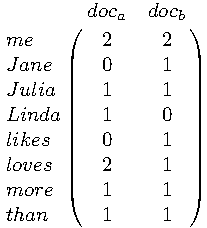
\includegraphics[width=0.25\textwidth]{images/TDMExample.pdf}
	\caption{An example of a Term-Document Matrix}
	\label{fig:TDMExample}
\end{wrapfigure}

The corresponding term-document matrix for $D$ is depicted in Figure \ref{fig:TDMExample}.

%The set of terms $t$ consists of $6$ elements, i.e. $t=(she$, $is$, $today$, $a$, $nice$, $city)$ and 

TDM has been exploited to characterize software systems and finally to compute similarities between them \cite{10.1109/APSEC.2004.69},\cite{10.1109ICPC.2016.7503721},\cite{McMillan:2012:DSS:2337223.2337267}. In a TDM for software systems, each row represents a package, an API call or a function and each column represents a software system. A cell in the matrix is the number of occurrence of a package/an API/function in each corresponding software system. A TDM for software systems has a similar form to the matrix shown in Figure~\ref{fig:TDMExample} where documents are replaced by software systems and terms are replaced by API calls.


\section{Cosine Similarity} \label{sec:CosineSimilarity}

Cosine similarity is a metric used to compute similarity between two objects using their feature vectors \cite{tversky1977features}. An object is characterized as a vector, and for a pair of vectors $\vec{\alpha}=(\alpha_{1},\alpha_{2},..,\alpha_{n})$ and $\vec{\beta}=(\beta_{1},\beta_{2},..,\beta_{n})$ there is an angle between them. Intuitively, the cosine similarity metric measures the similarity as the cosine of the corresponding angle between the two vectors and it is computed using the inner product as follows. 

\begin{equation} \label{eqn:Cosine}
CosineSim(\vec{\alpha},\vec{\beta}) = \frac{\sum_{i=1}^{n}\alpha_{i}\cdot \beta_{i}}{\sqrt{\sum_{i=1}^{n}(\alpha_{i})^{2} }\cdot \sqrt{\sum_{i=1}^{n}(\beta_{i})^{2}}}
\end{equation}

Figure \ref{fig:Cosine} illustrates the cosine similarity between two vectors $\vec{\alpha}$ and $\vec{\beta}$ in a three-dimension space. This can be thought as the similarity between two documents with three terms $t=(t_{1},t_{2},t_{3})$.

\begin{figure}[h!]
	\centering
	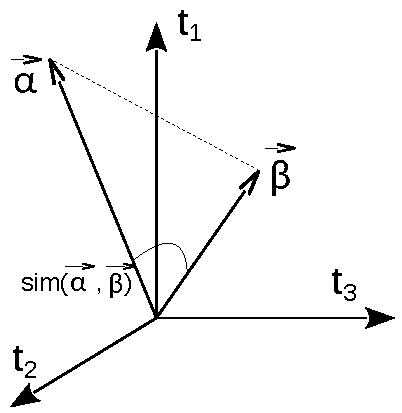
\includegraphics[width=0.25\textwidth]{images/Cosine.pdf}
	\caption{Cosine similarity between two feature vectors $\vec{\alpha}$ and $\vec{\beta}$}
	\label{fig:Cosine}
\end{figure}

Refer to the example in Section~\ref{sec:TDM}, the two documents are represented by means of two vectors as follows: 

%From the strings is possible to count the occurrencies of each term, putting everything in a matrix.
%Since in this kind of evaluation is not important the meaning or where the words are, is possibile to create the related vectore in order to compute the similarity.\\
%This is an example of how the cosine similarity can be done  between two sentences. These are the two string that we want to compare to see how much they are related each other.
%
	\begin{equation} \nonumber
	\vec{doc_a} = [2, 0, 1, 1, 0, 2, 1, 1]
	\end{equation}
	\begin{equation} \nonumber
	\vec{doc_b} = [2, 1, 1, 0, 1, 1, 1, 1]
	\end{equation}

And the similarity between them is computed using Equation~\ref{eqn:Cosine}: 

\begin{equation} %\label{eqn:Cosine}
CosineSim(\vec{doc_a},\vec{doc_b}) = \frac{9}{\sqrt{12}\cdot \sqrt{10}} = 0.822
\end{equation}

A similarity score of $0.822$ implies that these documents are highly similar.% each other 0.822, in a range between 0.0 and 1.0.

Cosine similarity has been popularly adopted in many applications that are related to similarity measurement in various domains \cite{Huang:2012:LCD:2343876.2343884},\cite{Islam:2008:STS:1376815.1376819},\cite{Linden:2003:ARI:642462.642471},\cite{conf:iscis:MadylovaO09},\cite{Mihalcea:2006:CKM:1597538.1597662}. Among the similarity metrics being recalled in this deliverable, the prevalence of Cosine Similarity is obvious as it is utilized in almost all of them as follows: \textit{MUDABlue} \cite{10.1109/APSEC.2004.69}, \textit{CLAN} \cite{McMillan:2012:DSS:2337223.2337267}, \textit{CLANdroid} \cite{10.1109ICPC.2016.7503721}, \textit{LibRec} \cite{6671293}, \textit{SimApp} \cite{Chen:2015:SFD:2684822.2685305}, \textit{WuKong} \cite{Wang:2015:WSA:2771783.2771795}, \textit{TagSim} \cite{Lo:2012:DSA:2473496.2473616}, and \textit{RepoPal} \cite{10.1109/SANER.2017.7884605}.


%%%%%%%%%%%%%%%%%%%%%%%%%%%%%%%%%%%%%%%%%%%%%%%%%%%%%%%%%  
%\section{Corpus-Based}




\section{Latent Semantic Analysis}

The problem with the term-document matrix is that the intrinsic relationships among different terms of a document cannot fully be captured. Furthermore, same words can be used to explain different requirements or the other way around, the same requirements can be described using different words \cite{10.1109/APSEC.2004.69}. Latent Semantic Analysis (LSA), also known as Latent Semantic Indexing (LSI), has been proposed to overcome these problems \cite{Landauer1998}. The technique exploits a mathematical model that can infer latent semantic relationships to compute similarity. LSA represents the contextual usage meaning of words by statistical computations applied to a large corpus of text. It then generates a representation that captures the similarity of words and text passages. To perform LSA on a text, a term-document matrix is created to characterize the text. Afterwards, Singular Value Decomposition (SVD) - a matrix decomposition technique - is used in combination with LSA to reduce matrix dimensionality \cite{kb2005}. SVD takes a highly variable set of data entries as input and transforms to a lower dimensional space but reveals the substructure of the original data. Essentially, it decomposes a rectangular matrix into the product of three other matrices as given in Equation ~\ref{eqn:Decomposition} \cite{kb2005}. Correspondingly, the decomposition is depicted in Figure~\ref{fig:Decomposition}.

\begin{equation} \label{eqn:Decomposition}
A_{mn}=U_{mm}S_{mn}V_{mn}^{T}
\end{equation}

in which

\begin{itemize}
	\item $U_{mm}$: Orthogonal matrix.
	\item $S_{mn}$: Diagonal matrix.
	\item $V_{mn}^{T}$: The transpose of an orthogonal matrix.
%	\item $X$: Low Rank matrix.
\end{itemize}


Figure~\ref{fig:Decomposition} depicts the low rank reduction phase. The new matrix is the product of the other three, but reducted, this is a very relevant issue. If the singular values in $S_{mn}$ are ordered by size, the first $k$ largest may be kept and the remaining smaller ones set to zero. The product of the resulting matrices is a matrix $X$ which is only approximately equal to $A_{mm}$ , and is of rank $k$. It can be shown that the new matrix $X$ is the matrix of rank $k$ which is closest in the least squares sense to $A_{mm}$. The amount of dimension reduction, i.e., the choice of $k$, is critical to our work. Ideally, we want a value of k that is large enough to fit all the real structure in the data, but small enough so that we do not also fit the sampling error or unimportant details. The proper way to make such choices is an open issue in the factor analytic literature. In practice, we currently use an operational criterion - a value of $k$ which yields good retrieval performance.%\\ In our work we decided a \emph{k value =} $\frac{repository}{2}$

\begin{figure}[h!]
	\centering
	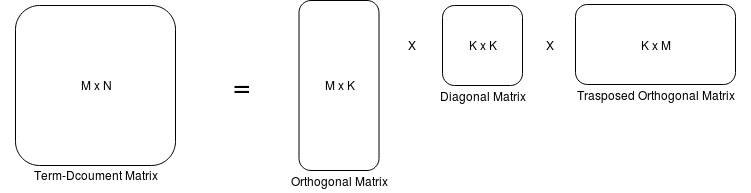
\includegraphics[width=15cm,height=20cm,keepaspectratio]{images/LSIk.png}
	\caption{The decomposition phase}
	\label{fig:Decomposition}
\end{figure}


$U_{mm}$ describes the original row entities as vectors of derived orthogonal factor values. $S_{mn}$ represents the original column entities in the same way, and $V_{mn}$ is a diagonal matrix containing scaling values. With the application of LSA it is possible to find the most relevant features and remove the least important ones by means of the reduced matrix $U_{mm}$. As a result, an equivalence of $A_{mm}$ can be constructed using the most relevant features. LSA helps reveal the latent relationship among words as well as among passages which cannot be guaranteed by a simple term-document matrix. The similarity measurement by LSA reflects adequately human perception of similarity and association among texts. Using LSA, similarities among documents are measured as the cosine of the angle between their row vectors (see Section~\ref{sec:CosineSimilarity}). LSA has been applied in \cite{10.1109/APSEC.2004.69},\cite{10.1109ICPC.2016.7503721},\cite{McMillan:2012:DSS:2337223.2337267} to compute similarities of software systems. The main disadvantage of LSA is that it is computational expensive when a large amount of information is analyzed.

%\newpage
%An example.

To illustrate how LSA works, we take an example with a set of $9$ documents as follows: %Image that these are a set of document to be analyzed and we want to apply the procedure stated before.

\begin{itemize}
	\item \textbf{doc}$_1$: \emph{Human machine interface for ABC computer applications.}
	\item \textbf{doc}$_2$: \emph{A survey of user opinion of computer system response time.}
	\item \textbf{doc}$_3$: \emph{The EPS user interface management system.}
	\item \textbf{doc}$_4$: \emph{System and human system engineering testing of EPS.}
	\item \textbf{doc}$_5$: \emph{Relation of user perceived response time to error measurement.}
	\item \textbf{doc}$_6$: \emph{The generation of random, binary, ordered trees.}
	\item \textbf{doc}$_7$: \emph{The intersection graph of paths in trees.}
	\item \textbf{doc}$_8$: \emph{Graph minors IV: Widths of trees and well-quasi-ordering.}
	\item \textbf{doc}$_9$: \emph{Graph minors: A survey.}
\end{itemize}

The term-document matrix for the document set is shown in Figure~\ref{fig:TermDocumentMatrix}.

\begin{figure}[h!]
	\centering
	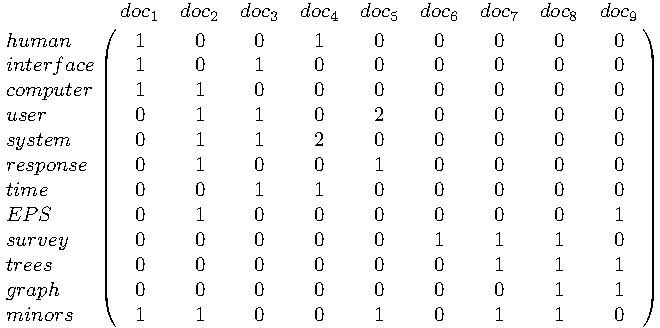
\includegraphics[width=0.8\textwidth]{images/TermDocumentMatrix.pdf}
	\caption{Term-Document Matrix of the example}
	\label{fig:TermDocumentMatrix}
\end{figure}

A computation exploiting an LSA implementation yields the matrices in Figures~\ref{fig:UmmMatrix},~\ref{fig:SmnMatrix}, and~\ref{fig:VmnMatrix}.Let's consider the \cite{Landauer1998} example to better explain how does the LSA works.

\begin{figure}[h!]
	\centering
	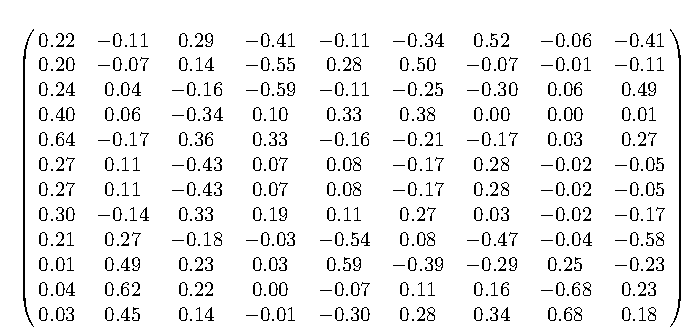
\includegraphics[width=0.8\textwidth]{images/UmmMatrix.pdf}
	\caption{Matrix $U_{mm}$x}
	\label{fig:UmmMatrix}
\end{figure}


\begin{figure}[h!]
	\centering
	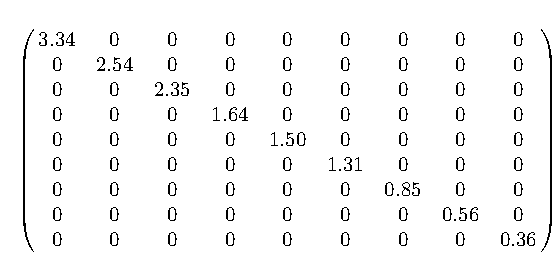
\includegraphics[width=0.68\textwidth]{images/SmnMatrix.pdf}
		\caption{Matrix $S_{mn}$}
	\label{fig:SmnMatrix}
\end{figure}


\begin{figure}[h!]
	\centering
	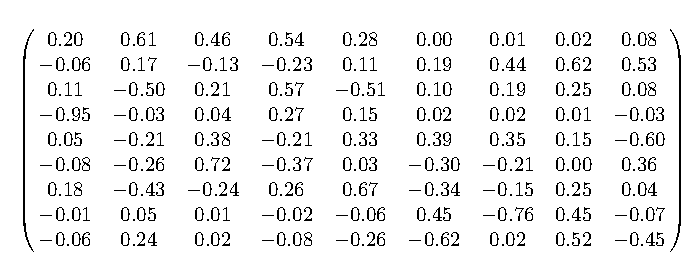
\includegraphics[width=0.8\textwidth]{images/VmnMatrix.pdf}
	\caption{Matrix $S_{mn}$}
	\label{fig:VmnMatrix}
\end{figure}

Figure~\ref{fig:DecomposedMatrix} depict the result of the decomposition with a rank of 2.

\begin{figure}[h!]
	\centering
	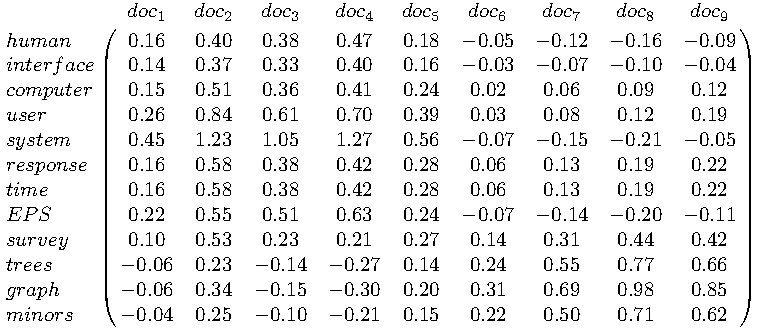
\includegraphics[width=0.9\textwidth]{images/DecomposedMatrix.pdf}
	\caption{The recovered matrix}
	\label{fig:DecomposedMatrix}
\end{figure}






\section{Jaccard Index}\label{sec:jaccard}

Given two objects $\alpha$ and $\beta$ represented by their corresponding set of elements $O(\alpha)$ and $O(\beta)$, the similarity is computed as the ratio of the cardinality of the intersection and the cardinality of the union of the two sets. The formula is given below:

\begin{equation} \label{eqn:Jaccard}
Jaccard(\alpha,\beta)=\frac{|O(\alpha)\bigcap O(\beta)|}{|O(\alpha)\bigcup O(\beta)|} 
\end{equation}

\begin{figure}[h!]
	\centering
	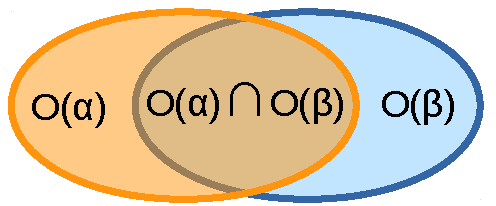
\includegraphics[width=0.4\textwidth]{images/JaccardSimilarity.pdf}
	\caption{Jaccard similarity between two sets $O(\alpha)$ and $O(\beta)$}
	\label{fig:Jaccard}
\end{figure}

The similarity using the Jaccard index is visualized in Figure \ref{fig:Jaccard}. The eclipse on the left hand represents $O(\alpha)$ and the eclipse on the right hand represents $O(\beta)$. The intersection of the two sets is $O(\alpha)\bigcap O(\beta)$ and the larger it is, the closer to $1$ is the Jaccard index. Once the two sets completely overlap each other, $Jaccard(\alpha,\beta)$ is equal to $1$. Among the similarity tools presented in this thesis, \textit{AnDarwin} \cite{Crussell2013} and \textit{RepoPal} \cite{10.1109/SANER.2017.7884605} employ Jaccard index in their implementation. %Furthermore, as a baseline for our evaluation, the index is used to compute similarity between two projects using their sets of dependencies (Section \ref{sec:CrossSimEvaluation}).



\section{Graph Similarity} \label{sec:GraphSimilarity}
Graph similarity is an active research field and receives a significant attention from the research community. In this section, we are going to review the approaches for computing similarity in graph that are beneficial to our context. A directed graph is defined as a tuple $G=(V,E,R)$, where $V$ is the set of vertices, $E$ is the set of edges and $R$ represents the relationship among the nodes. A graph consists of enormous nodes and oriented links with semantic relationships. A triple <$subject, predicate, object$> with $subject, object \in V$ and $predicate \in E$ states that node $subject$ is connected to node $object$ by means of the edge labelled with $predicate$. To evaluate the similarity of two nodes in a graph, their intrinsic characteristics like nodes, links, and their mutual interactions are incorporated into the similarity calculation \cite{DiNoia:2012:LOD:2362499.2362501},\cite{Nguyen:2015:CRV:2942298.2942305},\cite{Nguyen:2015:ESP:2740908.2742141}. Among others, feature-based semantic similarity metrics gauge the similarity between graph nodes as a measure of commonality and distinction of their hallmarks.

Tversky provides a deep insight into feature-based similarity in his work \cite{tversky1977features}. There, objects are represented as a set of common and distinctive features and the similarity between two objects is computed by comparing their features. An object is represented in one of the following forms: \emph{binary values}, \emph{nominal values}, \emph{ordinal values}, and \emph{cardinal values}. Feature-based semantic similarity metrics first attempt to characterize resources in a graph as sets of feature and then perform similarity calculation on them.

%Measuring similarity using features is based on the premise that the more common features two objects hold, the more similar they are. 
%Bearing on this principle, f
%the similarity between 

%In the following sub-sections, we are going to review three algorithms for computing similarity in graphs. These algorithms serve as base for our proposed approach that exploits the graph structure to compute similarity.

%\subsection{SimRank} \label{sec:SimRank}

\begin{figure}[h!]
	\centering
	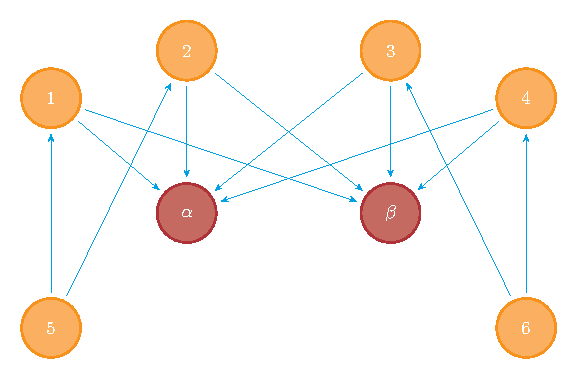
\includegraphics[width=0.60\textwidth]{images/SimRank.pdf}
	\caption{SimRank similarity}
	\label{fig:SimRank}
\end{figure}

SimRank has been designed to calculate similarity based on the mutual relationships between nodes \cite{Jeh:2002:SMS:775047.775126}. In a graph, the similarity between two nodes is dependent on their neighbors. Considering two nodes, the more similar nodes point to them, the more similar the two nodes are. For example, in Figure \ref{fig:SimRank}, the two nodes $\alpha$ and $\beta $ are highly similar because they are concurrently pointed by other four nodes in the graph. Also, node $1$ is similar to node $2$ since both are pointed by node $5$. Comparably, the similarity between node $3$ and node $4$ is high as they are pointed by node $6$. In this sense, the similarity between two nodes $\alpha$ and $\beta$ is computed by using a fixed-point function. Given $k \geq 0$ we have $R^{(k)}(\alpha,\beta) = 1$ with $\alpha = \beta$ and $R^{(k)}(\alpha,\beta) = 0$ with $k=0$ and $\alpha \neq \beta$. In all the other cases the general formula is:

\begin{equation}\label{eqn:SimRank}
R^{(k+1)}(\alpha,\beta) = 
\frac{\Delta}{|I(\alpha)|\cdot|I(\beta)|}\sum_{i=1}^{|I(\alpha)|}\sum_{j=1}^{|I(\beta)|}R^{(k)}(I_{i}(\alpha),I_{j}(\beta))
\end{equation}

where $\Delta$ is a damping factor ($0 \leq \Delta < 1$); $I(\alpha)$ and $I(\beta)$ are the set of incoming neighbors of $\alpha$ and $\beta$, respectively. $|I(\alpha)|\cdot|I(\beta)|$ is the factor used to normalize the sum, thus making $R^{(k)}(\alpha,\beta) \in [0,1]$. Equation~\ref{eqn:SimRank} implies that the similarity for two nodes is computed by aggregating the similarity of all possible pairs of their neighbors. 

SimRank has been used by \CrossSim  \cite{NDRDSEAA2018} as the mechanism to compute the similarity among nodes in a graph representing the OSS ecosystem.






%\clearpage
%%%%%%%%%%%%%%%%%%%%%%%%%%%%%%%%%%%%%%%%%%%%%%%%%%%%%%%%%%  
%\section{Knowledge-Based}
%Knowledge-Based Similarity aims to identify the degree of similarity between words using informations derived from semantic networks.
%Knowledge-based similarity measures can be divided roughly into two groups: measures of semantic similarity and measures of semantic relatedness.By semantic similarity we mean concepts that are related each other on the basis of their likeness.
%Semantic relatedness, on the other hand, is a more general notion of relatedness, not specifically tied to the shape or form of the concept. Semantic similarity is a metric defined over a set of documents or terms, where the idea of distance between them is based on the likeness of their meaning or semantic content as opposed to similarity which can be estimated regarding their syntactical representation (e.g. their string format).
%An example of relatedness is the Lask algorithm which identify senses of words in context using definition overlap. To clarify let's take a look an example in \cite{Resnik}.
%Using the Oxford Advanced Learner's Dictionary, it finds that word \emph{pine} has two senses:
%\begin{itemize}
%	\item{Sense 1: kind of \textbf{evergreen tree} with needle-shaped leaves}
%	\item{Sense 2: waste away through sorrow ir illness.}
%\end{itemize}
%
%The word \emph{cone} has three senses:
%\begin{itemize}
%	\item{Sense 1: solid body which narrows to a point}
%	\item{Sense 2: something of this shape whether solid or hollow}
%	\item{Sense 3: fruit of certain \textbf{evergreen tree}}
%\end{itemize}
%
%Each of the two senses of the word \emph{pine} is compared with each of the three senses of the \emph{cone} and it is found that the words \emph{evergreen tree} occurs in one sense each of the two words. These two senses are then declared to be the most appropriate senses when words \emph{pine} and \emph{cone} are used togheter.
%
%Concerning the similarity an example could be Resnik(1995) which uses the information content of concepts, computed from their frequency of occurrence in a large corpus, to determine the semantic relatedness of word senses\cite{Resnik}.
%Another example is Jian \& Conrath \cite{Jian}s It combines a lexical taxonomy structure with corpus statistical information so that the semantic distance between nodes in the semantic space constructed by the taxonomy can be better quantified with the computational evidence derived from a distributional analysis of corpus data. Specifically, the proposed measure is a combined approach that inherits the edge-based approach of the edge counting scheme, which is then enhanced by the node-based approach of the information content calculation.

